\chapter{Theoretical Appendix B: Metaphysical Arguments}
\section{Chance is not a valid explanation for biological phenomena; Randomness is a measure of property of sequences and not an explanation}
\label{sec:chance}
Substantial portions of this document are dedicated to an examination of Harris' regular invocation of ``stochastic" and related adjectives to describe the behaviour of RPCs. This is what lead me to characterise the theory primarily in those terms- the Stochastic Mitotic Mode Explanation. It may not be immediately obvious why this should be the case; most scientists assume that they know what words like ``stochastic" and ``random" mean well enough to use them in rigorous technical publications. We may not be aware that there has been a sprawling debate on the meaning of these terms since the earliest statistical formulations begain to appear in the 19th century. However, even the simplest examples (as current today as they were in Laplace's time) reveal how difficult this topic can be.

If we consider the classic example of the coin flip, a process whose outcome we generally regard as being in some way ``stochastic" or due to ``chance", we immediately face the question of whether these descriptions refer to our inability to know the outcome of the process, or whether they refer to properties of the process itself. In other words, if we could specify the mechanics of the coin toss with sufficient precision, could we predict the outcome? This reflects two possible senses in which we may legitimately describe a process as ``stochastic": referring to an epistemic dimension (we may describe some process as stochastic because we are unable to predict its outcome \textit{a priori}), or referring to an ontological dimension (we describe the process as stochastic because this, in some way, describes how it \textit{really is} independent of our knowledge of it).

Complicating matters is the sheer number of implications that we tend to associate with ``stochasticity" and ``randomness". We may be saying something about the causal structure of an event with deep metaphysical implications. It is common to distinguish between ``deterministic" and ``stochastic" processes, as though ``stochastic" literally meant ``indeterministic"- something like the Copenhagen interpretation of quantum physics. We may mean something about the apparent disorderliness of a series of outcomes of some process, with mathematical and information theoretical implications. What is an apparently simple observation- cellular fate distribution in RPC lineages is ``stochastic", now seems to require at least a little clarification or interpretation. In general, we may say that stochasticity, for Harris, applies to at least the following entities:

\begin{enumerate}
\item The population-level phenomenal outcome of the RPC fate specification process (the phenomenon itself)
\item The overall behaviour of the macromolecular system whose operations produces these outcomes (the macromolecular mechanism itself)
\item The particular behaviour of some component of the macromolecular system, eg. stochastic expression of transcription factors (the macromolecules themselves)
\item The statistical generalisations used to characterise relevant aspects of the behaviour of the mechanism or the macromolecules
\end{enumerate}

It is, moreover, hardly fair to expect Harris to be advancing a coherent theory about the ontological, objective basis of randomness or probability. Still, this leaves us in the awkward position of not knowing quite what the leading explanation for retinal formation is actually saying about its explanandum. The SMME is thus at risk of circularity- the explanandum (unpredictable variability in clonal outcomes) has as explanans a mechanistic explanation containing an abstract mathematical model tuned to produce this unpredictable variability. This may, in other words, turn out to be a convoluted case of \hyperref[fitting]{model overfitting}, if the ``stochasticity" in question does not have a material biological referent. Before considering this, we need to define our terms more carefully to avoid the pervasive confusion mentioned above.

\subsubsection{Chance versus Randomness}
A commonplace belief is that randomness refers to outcomes produced by chance events. In an extensive and useful discussion, Antony Eagle reviews the evidence for this Commonplace Thesis, or \textbf{(CT)}\cite{Eagle2018}, drawing on discussions in the physics literature. Importantly, he notes that chance and randomness are not identical, and that one can conceivably exist without the other. This, in effect, disproves the (CT)- it is very difficult to imagine how the two concepts can be directly related in this productive fashion. I will attempt a brief summary of Eagle's argument, with reference to Kolmogorov complexity:

Chance is mainly used to refer to processes. Exemplars are coin flips and die rolls. We can think of these as ``single-case" probabilities that we take to inhere in the process. For instance, we may say that an evenly weighted coin has a .5 probability of returning a value of heads on a flip, even if it is only flipped once. That is, probabilities can be taken to be objective properties of individual instances of processes, and not only descriptions of the frequencies of the process' outcomes over many repetitions. This is closely related to the logical concept of ``possibility". If something is possible, it has a chance of occurring. However, possibility is a logical binary; something is either possible or impossible. A ``single-case" probability is understood as something like an objective feature of a system as a whole given its actual configuration and the relevant natural laws.  

Randomness, by contrast, mainly refers to process \textit{outcomes}. That is, randomness is a property of a series of outcomes of multiple instances of some process. It turns out to be challenging merely to define what a ``random" binary sequence might be (perhaps generated by a series of coin flips). However, in general, we may say that a random sequence of outcomes is one that cannot be generated by an description shorter than the sequence itself. That is, there is no set of rules that can generate a genuinely random sequence from a shorter sequence. In algorithmic information theory, the length of the ruleset required to produce some piece of information (like a sequence of measured outcomes) is called the Kolmogorov complexity of that object; if the Kolmogorov complexity of the object is equal to the object's length, the object definitionally has the property of algorithmic or Kolmogorov randomness\footnote{The Kolmogorov complexity of a sequence can be estimated, contrary to common belief\cite{Li2008}. Minimum Message Length expresses a similar concept. More prosaically, one may simply compress a serialized representation of the sequence on one's hard drive with a reasonably good compression algorithm; the degree of compression achieved is a good indicator of the degree of non-random order available to shorten the sequence's description.}.

Eagle produces numerous examples of the dissociability of these concepts, from which I have selected two concise illustrations:

\begin{longquote}
Chance Without Randomness

...

A fair coin, tossed 1000 times, has a positive chance of landing heads more than 700 times. But any outcome sequence of 1000 tosses which contains more than 700 heads will be compressible (long runs of heads are common enough to be exploited by an efficient coding algorithm, and 1000 outcomes is long enough to swamp the constants involved in defining the universal prefix-free Kolmogorov complexity). So any such outcome sequence will not be random, even though it quite easily could come about by chance. 

...

Randomness Without Chance

...

Open or dissipative systems, those which are not confined to a state space region of constant energy, are one much studied class [of the objects of deterministic classical physics- notably, biological systems are dissipative], because such systems are paradigms of chaotic systems ... the behaviour of a chaotic system will be intuitively random ... [t]he sensitive dependence on initial conditions means that, no matter how accurate our finite discrimination of the initial state of a given chaotic system is, there will exist states indiscriminable from the initial state (and so consistent with our knowledge of the initial state), but which would diverge arbitrarily far from the actual evolution of the system. No matter, then, how well we know the initial condition (as long as we do not have infinite powers of discrimination)\footnote{Note that this condition defines chaotic randomness as an epistemic, rather than ontological, feature of complex systems- a being with infinite powers of discrimination could predict the evolution of a complex classical system with perfect accuracy.}, there is another state the system could be in for all we know that will evolve to a discriminably different future condition. Since this divergence happens relatively quickly, the system is unable to be predicted ... Just as before, the classical physical theory underlying the dynamics of these chaotic systems is one in which probability does not feature. 
\cite{Eagle2018}
\end{longquote}

Therefore, the (CT) is untenable. Processes are ``chancy"; collections of process outcomes, ``trials", or instantiations are ``random". It is tempting to say that Harris is explaining random fate outcomes with descriptions of chancy processes occuring internally to RPCs. Let us examine whether this is plausible. 

\subsubsection{Chance in molecular mechanisms}
I turn first to consider what it might mean to describe the behaviour of a biological macromolecular system as ``chancy". Let us again distinguish between the ontological and epistemic dimensions of this description. There is a sense in which the operation of a macromolecular mechanism could be said to be objectively chancy, and one in which the ``chancy" outcome reflects our ignorance of some source of variability in the process.

Eagle proffers two common lines of argument in favour of chanciness as an objective property of processes. The first is the notion of the ``single-case" probability mentioned above. The examples given are single coin flips, and the decay of single radioactive atoms, which are commonly taken to have chancy outcomes irrespective of anyone's beliefs about them. As Eagle notes, this is closely related to frequentist ideas about stable processes, or trials:

\begin{longquote}
It is the stable trial principle that has the closest connection with single-case chance, however. For in requiring that duplicate trials should receive the same chances, it is natural to take the chance to be grounded in the properties of that trial, plus the laws of nature. It is quite conceivable that the same laws could obtain even if that kind of trial has only one instance, and the very same chances should be assigned in that situation. But then there are well-defined chances even though that type of event occurs only once.

...

The upshot of this discussion is that chance is a \textit{process} notion, rather than being entirely determined by features of the outcome to which the surface grammar of chance ascriptions assigns the chance. For if there can be a single-case chance of $\frac{1}{2}$
for a coin to land heads on a toss even if there is only one actual toss, and it lands tails, then surely the chance cannot be fixed by properties of the outcome ‘lands heads’, as that outcome does not exist. The chance must rather be grounded in features of the process that can produce the outcome: the coin-tossing trial, including the mass distribution of the coin and the details of how it is tossed, in this case, plus the background conditions and laws that govern the trial. Whether or not an event happens by chance is a feature of the process that produced it, not the event itself. The fact that a coin lands heads does not fix that the coin landed heads by chance, because if it was simply placed heads up, as opposed to tossed in a normal fashion, we have the same outcome not by chance. Sometimes features of the outcome event cannot be readily separated from the features of its causes that characterise the process by means of which it was produced. 

\cite{Eagle2018}
\end{longquote}

Examining the example of the coin toss, we find a fairly simple answer to the question posed earlier: if we knew enough about the mechanics of the toss, could we predict its outcome? The answer is yes, we can- the Bell Labs statistician Persi Diaconis has built a coin tossing machine that reliably produces heads or tails \cite{Kestenbaum2004}. We therefore know that tightly controlling the mechanics of a coin toss allows us to treat this system as entirely deterministic, without any significant element of chance in the outcome. A coin toss is only chancy when the human doing it does not have full control over the mechanical parameters of the process. Conceptually, there is no \textit{a priori} reason why a coin-tosser should not be able to regularise the angular momentum of their thumb-flick by training with a strain gauge, place the coin on a stable surface allowing flicking, and achieve the same effect as the coin-tossing machine. In this case, Eagle's suggestion that ``[s]ometimes features of the outcome event cannot be readily separated from the features of its causes that characterise the process" seems obviously wrong- the ``chancy" element of coin tossing is fully separable from the rest of the coin tossing process, and replaceable with a non-chancy component.

If the foregoing argument is correct, it seems that the coin toss is an example of the epistemic, rather than ontological, dimension of chance. The process appears to be chancy, or random, because the human tossing the coin is not able to precisely control the mechanical parameters of the process. Indeed, as Diaconis notes, these epistemically-limited tossers do not actually produce unbiased random outcomes- human coin tosses come up as they were started slightly more often than with the obverse face \cite{Diaconis2007}.

Eagle's second example of an ``objective single-case chance", is the decay of a radioactive atom. This is a common method of making covert appeals to the second line of argument for objective chance, which is the existence of orthodox quantum theory. There is no known physical process whose parameters are thought to define the lifetime of individual radioactive atoms, in the way that there is a well-specified physical process that produces a particular coin toss outcome. Rather, this is an appeal to the Copenhagen theoretical principle that it is \textit{a priori} impossible to predict the lifetimes of individual atoms. As appeals to quantum theory to ground ``objective chance" in biological processes are becoming more common, let us consider whether a quantum theoretical explanation might plausibly underpin the ``stochasticity" of RPC fate specification.

\subsubsection{Can macromolecular chanciness be rooted in quantum indeterminacy?}
Eagle suggests that, because the Copenhagen interpretation of quantum physics has wide currency among physicists, the theory's implied indeterminacy of physical phenomena at the quantum level could ground ``objective chance". While common, this argument downplays the fact that quantum theory is not a homogenous scientific tradition. Unfortunately, a significant misrepresentation of the history of quantum theory has given rise to the impression that the Copenhagen theory is the unanimous or best articulation of quantum theory. We must briefly examine this misrepresentation before we can understand whether Eagle's argument makes sense.

The conventional history of mid 20th-century quantum theory holds that John Stewart Bell, in the demonstration of his famous inequality, conclusively proved that deterministic (so-called ``hidden variable") theories of quantum mechanics were incorrect. As demonstrated (strangely, without any acknowledgement) in another section of the very pages Eagle's argument appears in, this is a highly partisan and misleading view. Eminent Bohmian theorist Sheldon Goldstein conclusively demonstrates that Bell was an advocate of the deterministic Bohmian mechanical theory, and thought his famous inequality demonstrated that quantum phenomena could not be \textit{local}, not that they could not be \textit{deterministic}\cite{Goldstein2017}.

Indeed, Bohmian quantum mechanics are fully deterministic, describe all of the same phenomena as Copenhagen, and in several cases resolve problems that orthodox quantum theory cannot \cite{Goldstein2017}. We are not, therefore, facing unanimous expert consensus that there is objective chance at the quantum level. We rather have a situation where physical phenomena are  described by two different theory-sets, one of which takes its statistical generalisations to be descriptions of ontological indeterminacy (Copenhagen), and the other to reflect epistemic uncertainty about a determinate universe (Bohm). Moreover, there is no reason to prefer the Copenhagen approach, given that the Bohmian theory explains Copenhagen's paradoxical results ``without further ado"\cite{Goldstein2017}\footnote{Bizarrely, Copenhagen partisans claim that Bohmian mechanics is formally equivalent to the Copenhagen approach. If this is the case, chance is \textit{clearly} a function of model choices and not of any underlying ontological reality. However, Bohmian mechanics is, in fact, substantially more complete than its Copenhagen equivalent, which, by Eagle's (defective) logic, suggests reality is more likely to reflect the deterministic rather than the chancy approach.}, deals with empirically verified phenomena of physical and biological interest that Copenhagen does not (eg. electron tunneling), and was the preferred approach of the man who understood better than anyone his own results, J.S. Bell.

Therefore, Eagle's argument is incorrect. There is no reason to suppose that the existence of quantum theoretical models that posit objective chance is good evidence for the \textit{reality} of objective chance. Moreover, there are good reasons to suppose that the converse is true. In sum, then, we may say that there is no reason to consider Harris' argument to refer to \textit{objective, ontological} chance, since the arguments for the existence of both single-case objective chance or quantum chance are weak and biologically irrelevant. Clearly, however, the \textit{epistemological} dimension of chance is in play here.

\subsubsection{Randomness in RPC fate specification}

Having dealt with how the concept of chance might apply to Harris' SMME above, let us consider how the term ``random" might relate to the process of RPC fate specification and differentiation. As introduced earlier, the technical meaning of ``randomness" pertains to sequences of process outcomes. The process outcomes Harris is concerned with are the temporally-arranged fate outcomes of some particular RPC lineage. Therefore, we must ask whether these sequences meet any reasonable technical definition of ``random".

Harris' own model proves that RPC fate outcomes are not algorithmically random. That is, the sequence of outcomes has a structure that can be meaningfully compressed by rules which produce typical RPC fate outcomes (Harris' mathematical models are such rule sets). One might object that Harris' meaning is that the particular rules which give rise to cellular fate ``choice" in his models involve random number generation. In this case, the claim is trivially about the model and not about the sequence of outcomes that is actually observed in zebrafish eyes. Indeed, all of Harris' later models \textit{axiomatically assume} a tripartite temporal structure to the differentiation process\footnote{That is, an early bias in RPC production is produced in these models by the a priori commitment to a ``rule" which results in early RPC production.}. This is precisely the type of sequential bias which allows efficient compression of a non-random sequence of outcomes by an algorithm. Therefore, Harris himself concedes that RPC fate specification is not an algorithmically random process\footnote{Having debunked the lay sense of ``random" being equivalent to ``chancy" above, there is no reason to consider these other, confused, non-technical definitions of randomness. They are neither logically defensible nor practically quantifiable, and therefore are of no scientific interest.}.

We should further note that the question of how predictably ordered, i.e. non-random processes like fate specification arise in biological systems is a fundamental question of the biological sciences. It has long been recognised that classical and quantum physical systems which have algorithmically random initial conditions do not spontaneously evolve to a state of order. In many ways, then, it is the extent to which variable sequences of outcomes like RPC fate specification \textit{depart} from algorithmic randomness which of interest when we are asking questions like ``how does the ordered structure of a retina arise from RPC activity?"

\subsubsection{Summary: ``Stochastic" or ``variable"?}

Above, I argue that the RPC fate specification process is not objectively chancy (since objective chance is an empirically unsupported concept), nor random (since the sequence of RPC lineage outcomes is structured and therefore non-random). What, then, should we make of the argument that this process is ``stochastic"? Let us consider the forceful argument of the great Bayesian statistician Edwin Thompson Jaynes:

\begin{longquote}
 ``Belief in the existence of ‘stochastic processes’ in the real world; i.e. that the property of being ‘stochastic’ rather than ‘deterministic’ is a real physical property of a process, that exists independently of human information, is [an] example of the mind projection fallacy: attributing one’s own ignorance to Nature instead. The current literature of probability theory is full of claims to the effect that a ‘Gaussian random process’ is fully determined by its first and second moments. If it were made clear that this is only the defining property for an abstract mathematical model, there could be no objection to this; but it is always presented in verbiage that implies that one is describing an objectively true property of a real physical process. To one who believes such a thing literally, there could be no motivation to investigate the causes more deeply than noting the first and second moments, and so the real processes at work might never be discovered. This is not only irrational because one is throwing away the very information that is essential to understand the physical process; if carried into practice it can have disastrous consequences. Indeed, there is no such thing as a ‘stochastic process’ in the sense that the individual events have no specific causes." \cite{Jaynes2003}
 \end{longquote}
 
It is important to emphasize that the utility of stochastic modelling techniques should not be taken to suggest that on some level the modelled phenomenon is actually, i.e. irreducibly, random and without causal structure. When speaking of biological ``randomness" or ``stochasticity", biologists rarely precisely define what is meant by these terms. This vagueness sometimes arises from, or results in, a theoretical deficit where properties of statistical models are understood to directly reflect the system being modelled; the scientist has failed to heed Korbzysky's dictum insisting that ``a map \textit{is not} the territory it represents, but, if correct, it has a \textit{similar structure} to the territory, which accounts for its usefulness" \cite{Korzybski2005} (italics in original). The ``structural similarity" here is between the model's outcomes and the collection of actually-observed population outcomes, \textit{not} the underlying biological process giving rise to measured outcomes. I conclude by suggesting that this particular example applies to all such explanations in the biological sciences. There is presently no good reason to accept scientific explanations rooted in chance. As for explanations rooted in randomness, to be credible, these must actually estimate the degree of randomness present in the relevant outcomes, and explain departures from pure incompressibility.


\section{Macromolecular mechanistic explanations in the Systems era}

The data chapters of this thesis are concerned with two issues in scientific practice: the comparison of models with different structures, and their interpretation. I began my career in stem cell biology with a background in molecular pharmacology, and the particular explanatory worldview that training inscribed. For me, biological explanation was about elucidating mechanisms, which consisted of descriptions of macromolecules and their accessory small molecule messengers interacting. "Models," in the sense of numerical simulations susceptible to formal statistical testing, were only the formal encoding of a body of knowledge that was first proved out at the bench, in interventional experiments. That these results could be encoded by a system of differential equations (SODE) only confirmed the rigour of the original analysis which composed the mechanistic explanation in the first place. That engineers should bring their (allegedly) sophisticated numerical techniques into our laboratories, only to have their expert analyses confirm the plain-sense interpretations of the benchworkers producing the data, served to reinforce the sense that the pharmacological approach was fundamentally the correct one. It hardly ever entered our minds that model comparison was not occurring at all; it seemed that null hypotheses had already been slain by the flurry of t-tests and ANOVAe applied to the underlying datasets before the eggheads showed up.

That there were problems with this approach was already apparent by the beginning of my graduate education; Faculty of Medicine graduate pharmacology seminars in the early 2000s routinely included dark warnings about the collapse of antidepressant effect sizes over time, and the need for new statistical approaches. Reports that most biomedical research results are not replicable were met with a sort of palpable relief \cite{Ioannidis2005}, if not much practical change. Ultimately, the power of the macromolecular mechanism in pharmacology proved overstated; the productivity lull of the 2000-2010 era has been overcome not by rational mechanistic design of traditional small molecules, but by an influx of new classes of drugs, often with unknown or poorly characterised mechanisms of action \cite{Munos2019}. The arrival of new statistics has not helped matters much; serious Bayesian analyses tend to doubt whether medical pharmacological interventions are effective at all \cite{Stegenga2018}. Still, by the time I had left for greener pastures with the stem cell biologists at the new Department of Cell and Systems Biology, it was clear that the pharmacological view of biological explanation had won significant discursive battles.

A fascinating artefact of this discursive victory is present in the best available study on the use of mechanistic explanations in stem cell biology, Melinda Fagan's "Philosophy of stem cell biology: knowledge in flesh and blood". In concluding chapters outlining the future of stem cell biology, Fagan provides a diagrammatic summary of what she takes to be the field's consensus on its general direction into its future ``Systems Biology'' incarnation, which I reproduce here in \autoref{faganSystems}.


\begin{wrapfigure}{l}{0.4\textwidth}
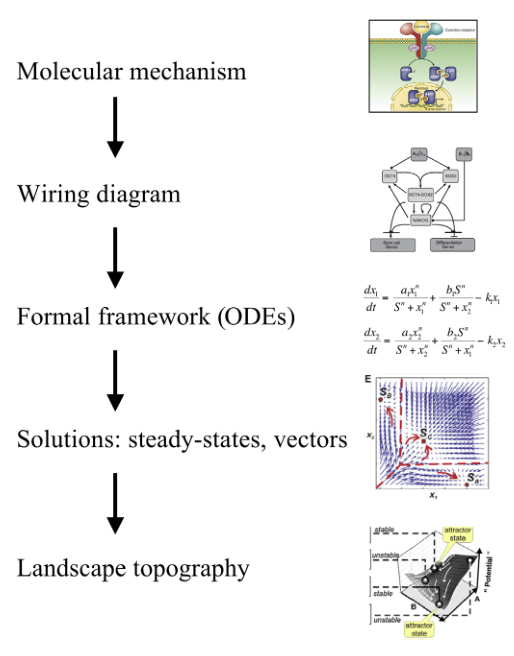
\includegraphics[scale=.36]{Fagansystems}
\caption{Cellular systems model-construction, excerpted from \cite[p.7]{Fagan2015}. The system of equations and subsequent steps are based on a 2-element wiring diagram.}
\label{fig:faganSystems}
\end{wrapfigure}

The perspicacious reader will observe that this is nothing other than the pharmacological view I outline above: the practice of molecular biology is the elucidation of mechanisms, the practice of systems biology is the formalization of these mechanisms as systems of differential equations. What was most peculiar about the presence of this view is that it makes no account of the Simple Stochastic Model, which receives significant coverage elsewhere in the book. This was particularly important to me because I was trying to understand how to use Harris' models to explain my results. What Harris was doing was clearly intended to be both a mechanistic explanation, in the sense that it eventually nominated a pair of particular transcription factors as the causative agents, and also a Systems explanation, in the sense that it relied, for persuasive effect, on complex numerical modelling techniques. It was formulated in SSM terms, however, not as a SODE, and critically was about the interpretation of a mathematical construct, not about the joint action of the named macromolecules, as Fagan suggests we should understand mechanistic explanations \cite{Fagan2013}.

Moreover, much of the sophisticated literature on mathematical models of stem cell variability are based on interpretations of dynamical systems theory or chaos theory \cite{Furusawa2012,Huang2017} that deal with the macromolecular constituents of cells as bulk expression values; that is, a protein may be represented in one of these models as a coordinate on an dimension representing the amount of the protein expressed. It is extraordinarily rare for these models to be very concerned about crystal structures, phosphorylation states, or any of the other mechanistic details the pharmacological view is so concerned with. Other approaches rely on control systems theory \cite{Sun2015,Yang2015a}, many other gaily use technical information-theoretic terms like ``noise'' without any effort to define or measure it \cite{Chang2008}, still others treat the expression of macromolecules as the endpoints of tissue-mechanical forces \cite{Peng2017}, and so on. The actual variety of ``systems'' explanatory strategies found ``in the field'' is bewildering; to become proficient in even one is a years-long project. As I began to grasp the sheer number of technical and theoretical subdomains implicated in these explanations, the full force of Nicholas Reschers' argument on this point became apparent: 

\begin{longquote}
The ramifications and implications of philosophical contentions do not respect a discipline's taxonomic boundaries. And we all too easily risk losing sight of this interconnectedness when we pursue the technicalities of a narrow subdomain. In actuality, the stance we take on questions in one domain will generally have substantial implications and ramification for very different issues in other, seeming unrelated domains. And this is exactly why systematization is so important in philosophy - because the way we \textit{do} answer some questions will have limiting repercussions for the way we \textit{can} answer others. We cannot emplace our philosophical convictions into conveniently delineated compartments in the comfortable expectation that what we maintain in one area of the field will have no unwelcome implications for what we are inclined to maintain in others.
\cite[p.97]{Rescher2005}
\end{longquote}

Indeed, the sudden injection of the philosophical contents of the ``complexity sciences'' into biological discourse felt like an invasion; suddenly, it was not very clear what a mechanism or a biological explanation might consist of after all. Michel Morange has argued persuasively that molecular biology is essentially mature \cite{Morange2003} and that "systems" explanations consist mainly in the complementation of ordinary molecular practice with sophisticated mathematical models \cite{Morange2008}, while acknowledging the increasing space available for the entry of physical explanations in molecular biology \cite{Morange2011}. This account is appealing, but it belies the chaotic nature of the recent scientific scene, and cannot make sense of why there are so many contending, often quite incompatible, views on how to explain cellular and molecular biological phenomena and why so few of those views include any idea on \textit{how those explanations might be tested against one another}.

\subsection{The Feyerabendian modeller}
\label{sec:Feyerabend}
\autoref{chap:SMME} cites Paul Feyerabend in establishing that scientific theories proceed by making metaphysical claims about reality. This point informs the model-analysis in that chapter, highlighting the sense in which the entities to which the Stochastic Mitotic Mode Explanation (SMME) refer become progressively more abstract and restricted to the mitotic mode concept. Mitotic mode is not a physical existent, but rather an abstraction compounding the fate of multiple cells- it is in this sense plainly meta-physical. Feyerabend has a number of essential insights on scientific metaphysics, which, when taken on board, allow us to make sense of what is happening within stem cell biology and more broadly, in the ``systems biology'' era. The central, seminal insight of Paul Feyerabend's \textit{Against Method} is that the observed historical succession of scientific theories occurs by counterpositional advancement of incompatible opposing theories, because only counterinductive comparisons \textit{between} theories are capable of showing up their implicit assumptions and allowing them to be challenged. Feyerabend explains:

\begin{longquote}
... it emerges that the evidence that might refute a
theory can often be unearthed only with the help of an incompatible
alternative: the advice (which goes back to Newton and which is still
very popular today) to use alternatives only when refutations have
already discredited the orthodox theory puts the cart before the
horse. Also, some of the most important formal properties of a theory
are found by contrast, and not by analysis. A scientist who wishes to
maximize the empirical content of the views he holds and who wants
to understand them as clearly as he possibly can must therefore
introduce other views; that is, he must adopt a \textit{pluralistic methodology}.
He must compare ideas with other ideas rather than with
'experience' and he must try to improve rather than discard the views
that have failed in the competition.\cite[p.20]{Feyerabend1993}
\end{longquote}

Feyerabend is interested in debunking the notion that science differs from other discursive social practices by showing that no universal method vouchsafes the progressive replacement of earlier, inferior theories with later, improved ones. He famously establishes that Galileo used a form of metaphysical propaganda, particularly in the ad hoc invocation of the now-discredited concept of circular inertia, to establish the credibility of the Copernican model against its orthodox Aristotlean competitor championed by the Catholic Church. Although we commonly think of the so-called Copernican Revolution as the replacement of an obviously defective theological explanation by a properly formed theory from the empirical sciences, Feyerabend shows that this conceals the actual means by which Galileo makes his persuasive case for the (itself badly defective) Copernican model.  Galileo's theory substantially contradicted the available evidence, erroneously asserted the reliability of some telescopic observations and discredited others\footnote{Galileo asserted that comets are optical illusions, for instance, since their non-circular orbits disconfirm the Copernican system, which insists on the circularity of orbital motion.}, made extensive use of ad hoc hypotheses, and was advanced by propagandistic and even dishonest means. Much of this was unavoidable. Ad hoc hypotheses are necessary for new theories because the auxiliary sciences associated with them have not been developed- scientific development is intrisically uneven, obligating the use of these makeshift theoretical devices. Without a certain level of dishonesty and rhetorical sleight of hand on Galileo's part, the Copernican program would have succumbed to the greater development and argumentative weight of the scholastic tradition. As Feyerabend notes, if any of the typically suggested criteria for a universal scientific method were applied, the Church would have won the debate and we might still have an Aristotlean cosmology. Much the same can be said in the case of Einstein or Bohr's scientific programmes, both scientists viewing themselves as outsiders attacking an established orthodoxy.

Because of his concern to attack what he sees as the overweening social influence of scientific and technical experts, Feyerabend puts a great deal of emphasis on the discursive process of establishing orthodoxy within a field, and the sense in which this is common to scientific and nonscientific domains. That is, the practice of the natural sciences are susceptible to the same irreducibly subjective and historically contingent social, political, economic, etc. forces as all other domains of human culture, and in this sense there is nothing special about scientific practice that shields its conclusions from error introduced by these means. These extra-scientific forces have significant effects on the forms scientific models take and the interpretations they are given, and it helps to remember this when reading modelling papers published to, in effect, keep the lights on. Still, I suggest that it is important not to interpret these arguments too pessimistically. Feyerabend genuinely wanted to promote what he called "Open Exchange" between different scientific and metaphysical traditions, centered around a noncoercive exchange of, in effect, models and standards for judging them. He was also wrong that there is nothing particular to the practice of natural sciences that is not present in other domains of human activity; statistical descriptions of collections of outcomes and of uncertainty, and a self-reinforcing dynamic of scaffolding methodological complexity, are unique to the modern natural sciences.

Ultimately, the value in Feyerabend's perspective is seeing that scientists routinely operate as epistemological anarchists, finding what works in their local institutional surroundings, and that we must expect that this will be the case. In other words, Fagan's (extremely carefully argued) conceptualization of the orthodox molecular mechanism, as found in stem cell biology, is useless for interpreting Harris' theories. This is so because Harris does not care about adhering to this standard of orthodoxy. The field has, in typical anarchic fashion, begun adapting models from a panoply of engineering, physics, statistical mechanics, AI, etc. subdisciplines, more or less willy nilly, and often without any sort of analysis of the adequacy of the model relative to alternatives. Moreover, these models pertain to a variety of levels of biological organisation, from the tissue down to subcellular nuclear compartments, and frequently do not refer in any concrete way to biological macromolecules.

I argue that, from this point of view, the macromolecular mechanistic explanation Fagan reifies is, in fact, already dead. The era of painstaking, effector-by-effector construction of macromolecular pathways, to be virtually enshrined in their ultimate SODE incarnation, perhaps ultimately to be assembled into some Monodian model cell-as-cybernetic-factory, is over, if it ever existed. This is not to say that Morange is wrong- as he asserts, molecular biology is not dead, it has not been replaced by ``systems biology''. In practice, however, the traditional form of molecular biological explanation is rapidly being replaced by explanatory forms from other fields, and it is not always clear that this has been salutory. For Feyerabend, science, like other human social practices consists of a variety of interacting traditions with differing assumptions, methods, sensory interpretations, and so on. The development of science is thus ``not the interaction of a practice with something different and external, \textit{but the development of one tradition under the impact of others.}" \cite[p.232]{Feyerabend1993}. The concept of ``systems biology'' is fundamentally an artefact of the impact of advanced statistics and statistical mechanics on biology. The resolution to the question of how this impact is mediated will determine the institutional and intellectual landscape that results from it. 

To have any agency in this process, molecular biologists must be able to assess the theoretical contents that are being imported into our field for ourselves. If we do not, we cannot assess the impact of the metaphysical commitments of these theories on the rest of our theorising, as Rescher persuasively insists that we must. Indeed, it was Feyerabend's perspective that led me to realise that there were at least three scientific orthodoxies hindering me from understanding the metaphysical contents of Harris' theories. These were the mechanism-to-SODE pipeline instilled by my pharmacological training and recapitulated by Fagan, the mendacious insistence on the actual reality of chanciness by Copenhagen theorists, and the broken and illogical statistical approaches commanded by frequentist statisticians. By realising that any conceptual element could appear in a mechanistic explanation, by rejecting the objective reality of chance, and embracing the original formulation of statistical orthodoxy suggested by LaPlace (that is, Bayesian statistics), I was able to counter-inductively show up the fundamental problems with Harris' theory.

Moreover, by the conscious adoption of Bayesian methods from cosmology to address local problems in stem cell biology, I attempt to model Feyerabend's Open Exchange between two scientific traditions. My selection of Skilling's nested sampling system of inference is driven by my appreciation for its logical consistency, simplicity, deep roots in fundamental logic and information theory, and broad applicability to a wide range of problems. While Feyerabend is no doubt correct that, ultimately, the selection of criteria to distinguish between scientific theories must itself be subjective, the deep comportment of Skilling's system with the fundamental human drive toward cognitive harmony \cite{Rescher2005} compels me to suggest that it may serve as a near-universal yardstick of the adequacy of scientific models with respect to their underlying datasets in the not-too-distant future.